\subsubsection{Company}
Companies can also register with CPP and there are two levels of approval a company may reach:
  \begin{enumerate}
    \item Advertisement of events and placements only, which any company should be allowed to do.
    \item Advertisement of events and placements and access to students (including emails), to be given to Corporate Partners of Imperial.
  \end{enumerate}
  In the following example a recruiter from Amazon, Sally, wishes to sign up in order to find talented students for placements and a complete example of a profile can be seen below for reference.
  \begin{figure}[H]\centering
  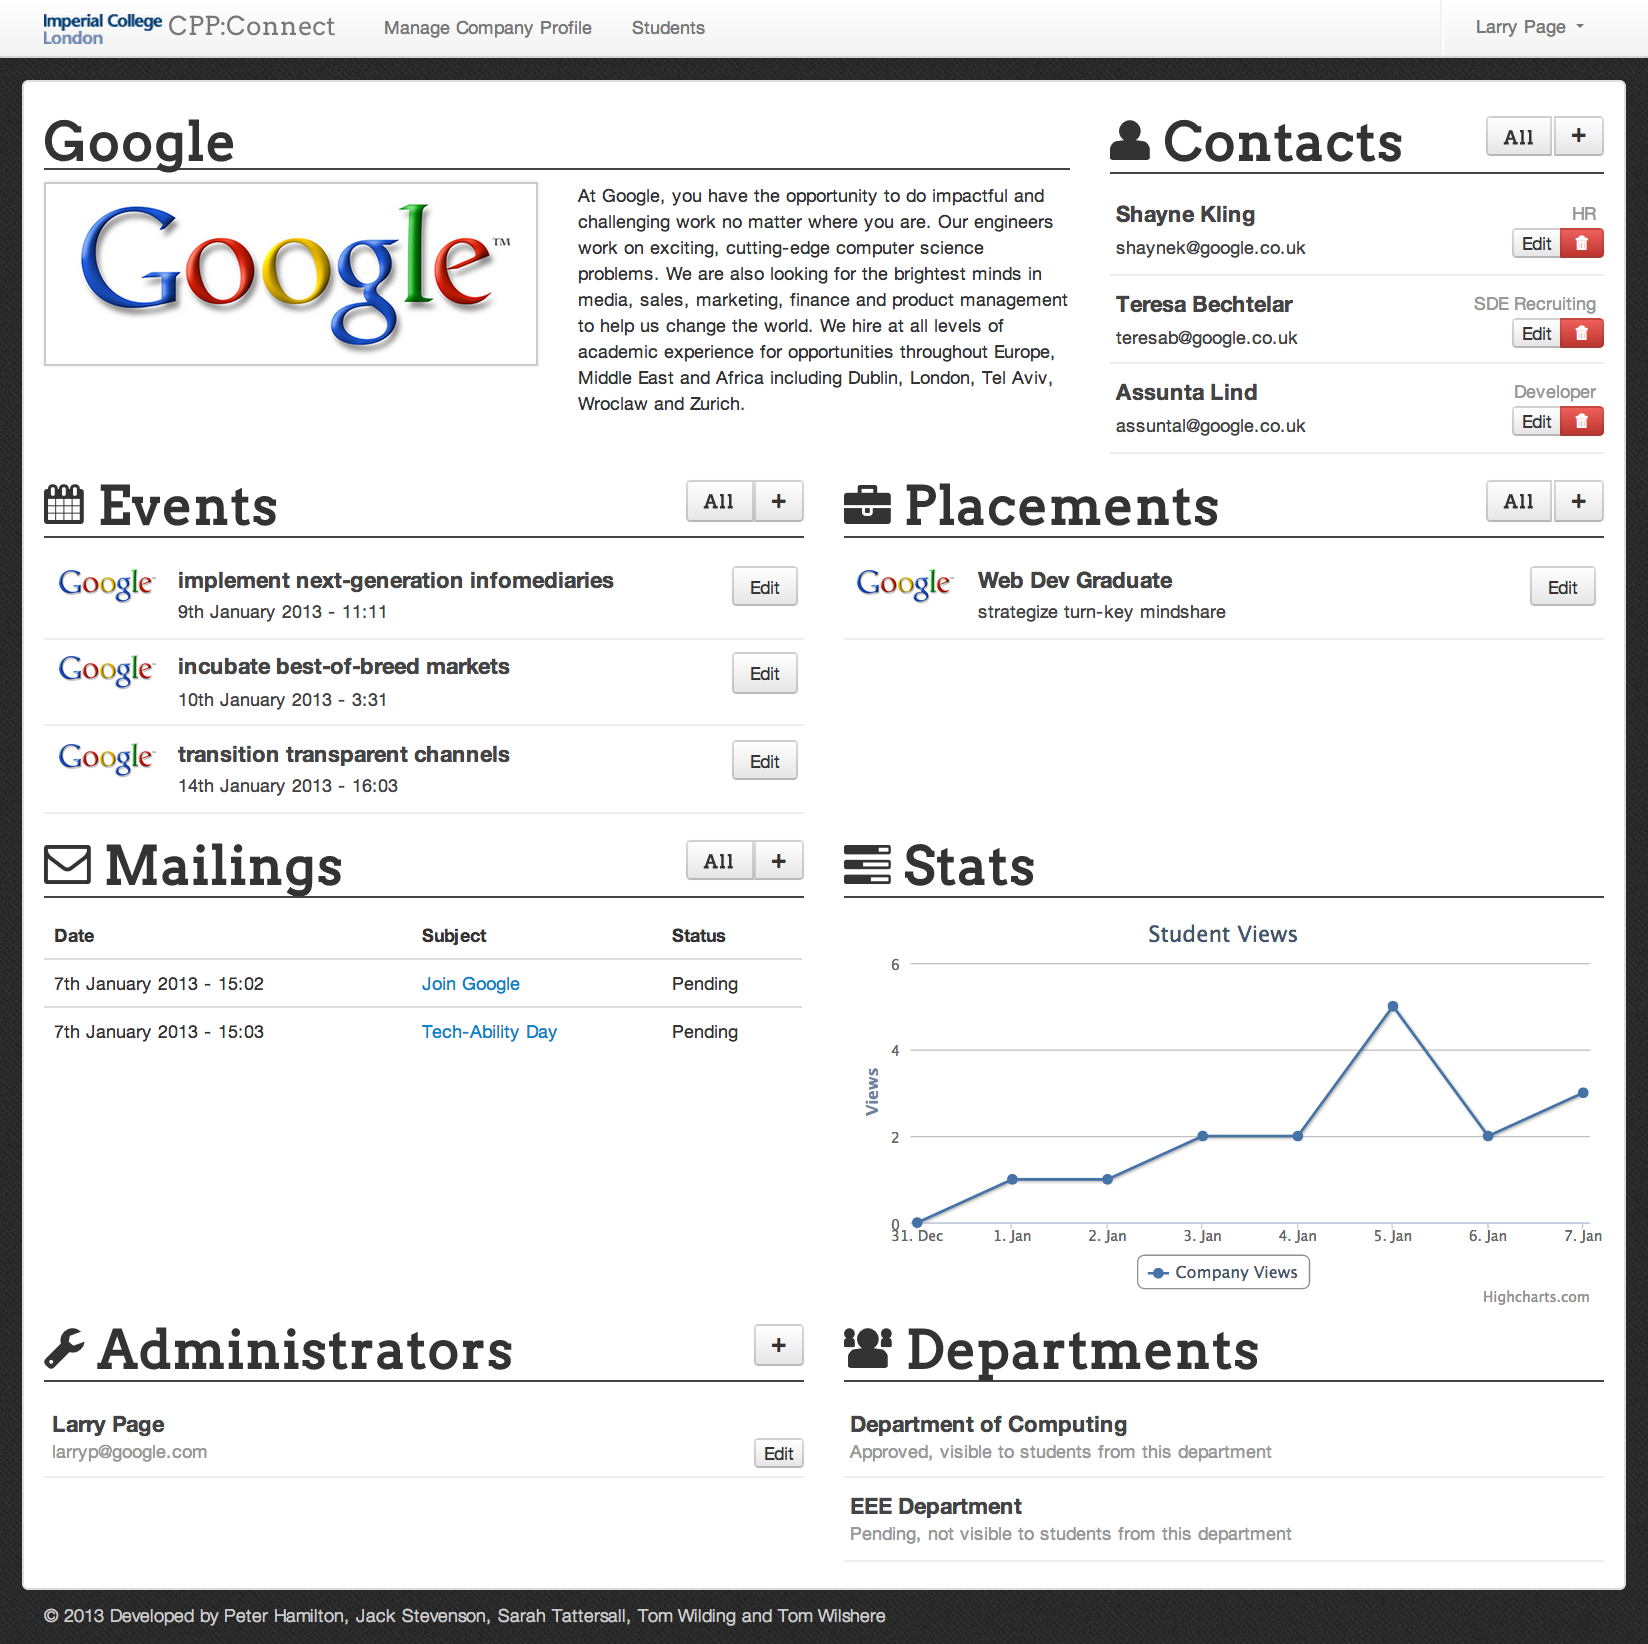
\includegraphics[scale=0.5]{images/user_experiences/company/complete_company_profile}
  \caption{A complete company profile}
  \end{figure}


  \paragraph{Sign up:}  
    If Amazon had not yet registered as a company, then Sally must sign up on the companies behalf using the clear and concise sign up page.

    \begin{figure}[H]\centering
    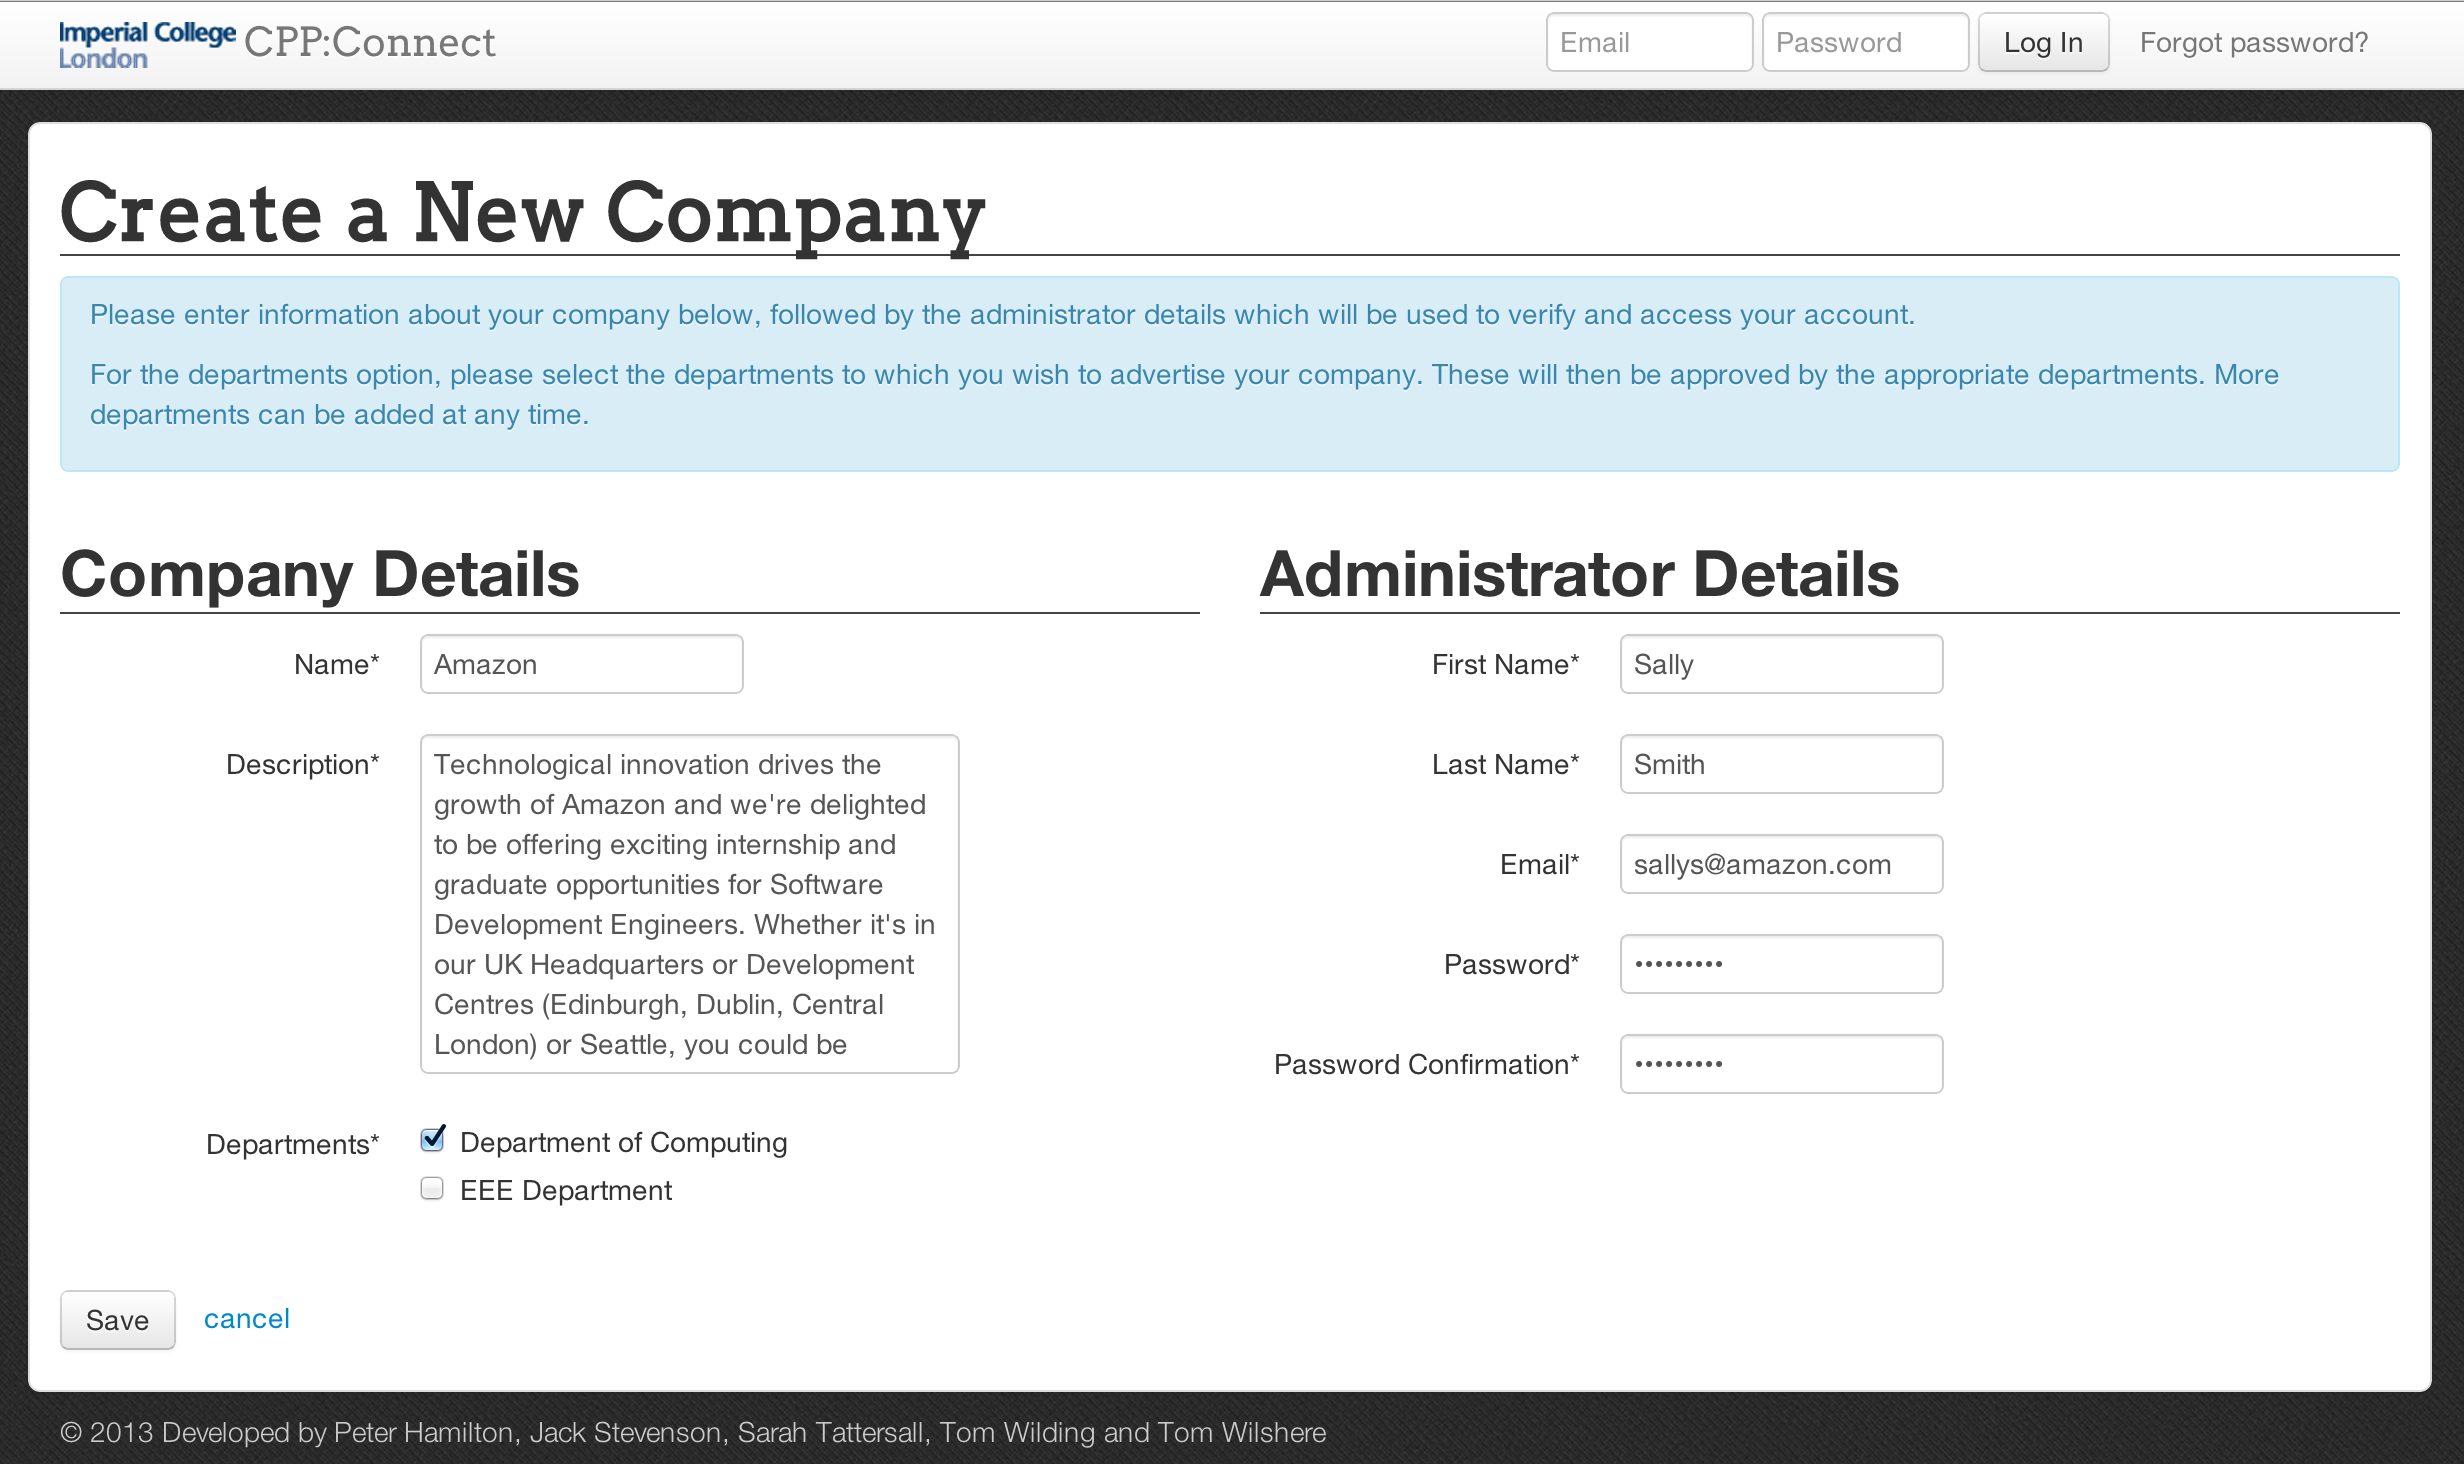
\includegraphics[scale=0.3]{images/user_experiences/company/amazon_signup}
    \caption{Company sign up page}
    \end{figure}

    Since our website is public administrators may not want some companies to be given access to the site. As such, as soon as a company has registered they are put into a holding state pending approval by an administrator.
    The basic level of approval is free, however access to students will only ever be granted to the Corporate Partners, who invest money in our department - since we need to give them some incentive to pay!

    Whilst waiting for administrator approval they can still edit their profile and create events and placements, but none of these will show up to students until approval is granted. They are notified whether approval has been gained via the departments section on their dashboard.

  \paragraph{Dashboard}
    Once signed in Sally is relocated to her dashboard, which has the same useful tool tips and extra features as the student page.

    Sally would like to add another administrator, Jeff, to help her balance her work load and she can easily do this by clicking on the new administrator button. We decided that administrators have the right to delete other administrators but not themselves to prevent them from being locked out forever. It will also mean that if the company only has one administrator they cannot be deleted which would then leave the company stagnant.

    \begin{figure}[H]\centering
    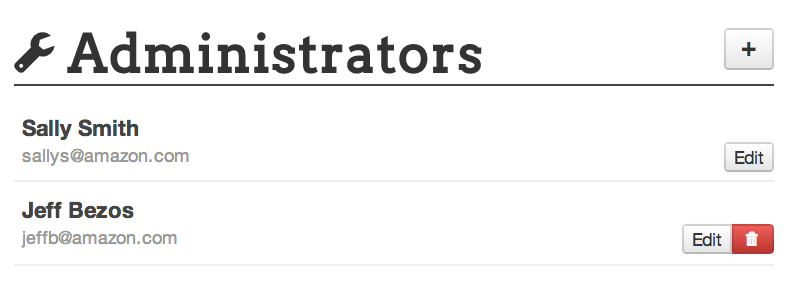
\includegraphics[scale=0.5]{images/user_experiences/company/jeff_admin}
    \caption{Signing a company administrator up is very easy}
    \end{figure}

    Sally can also see how many students have viewed Amazon's profile, a low number is likely to indicate they are not advertising enough events and/or placements and so their presence on the site is lacking appeal.

    \begin{figure}[H]\centering
    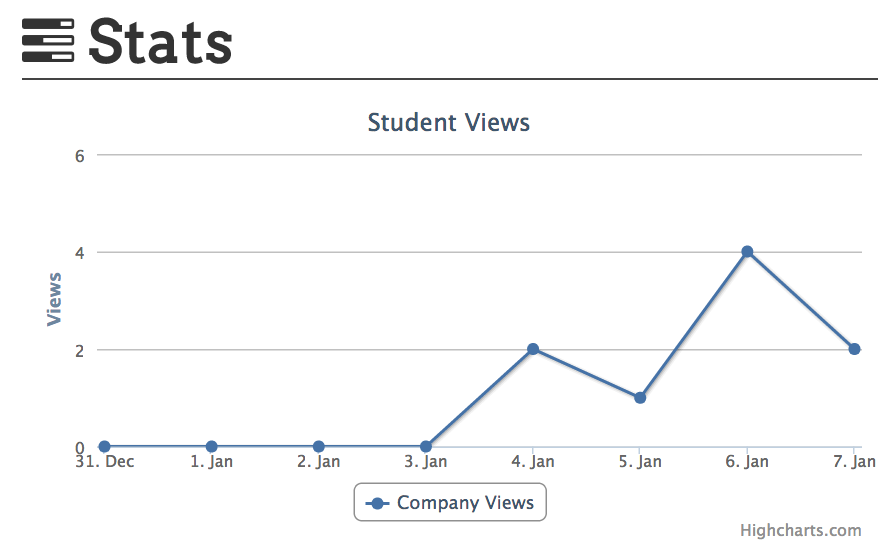
\includegraphics[scale=0.5]{images/user_experiences/company/stats}
    \caption{Company view statistics}
    \end{figure}

  \paragraph{Contacts:}
    Sally decides that she wishes students to be able to contact her regarding job opportunities so adds her details to the company contacts in the top right hand corner of the dash board. This very nicely comes up with an in place form for Sally to fill out.
    She fills out her details and notices that once she's added contacts she can drag and drop them to re-order the list.

    \begin{figure}[H]\centering
    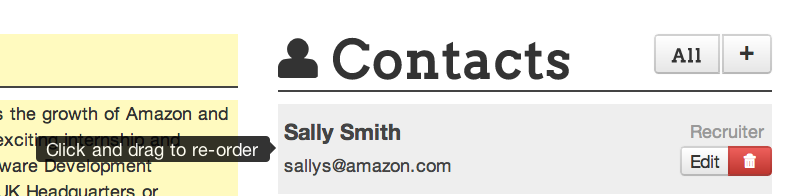
\includegraphics[scale=0.6]{images/user_experiences/company/contact_drag_and_drop}
    \caption{Tooltip for company contacts}
    \end{figure}

  \paragraph{Events and Placements:}
    Sally decides that it might be a good idea to post that Amazon is offering six month industrial placements and so clicks on the new placement button.
    She receives important notices from the departments she's registered to that she reads and makes note of and then proceeds to create the placement.

    \begin{figure}[H]\centering
    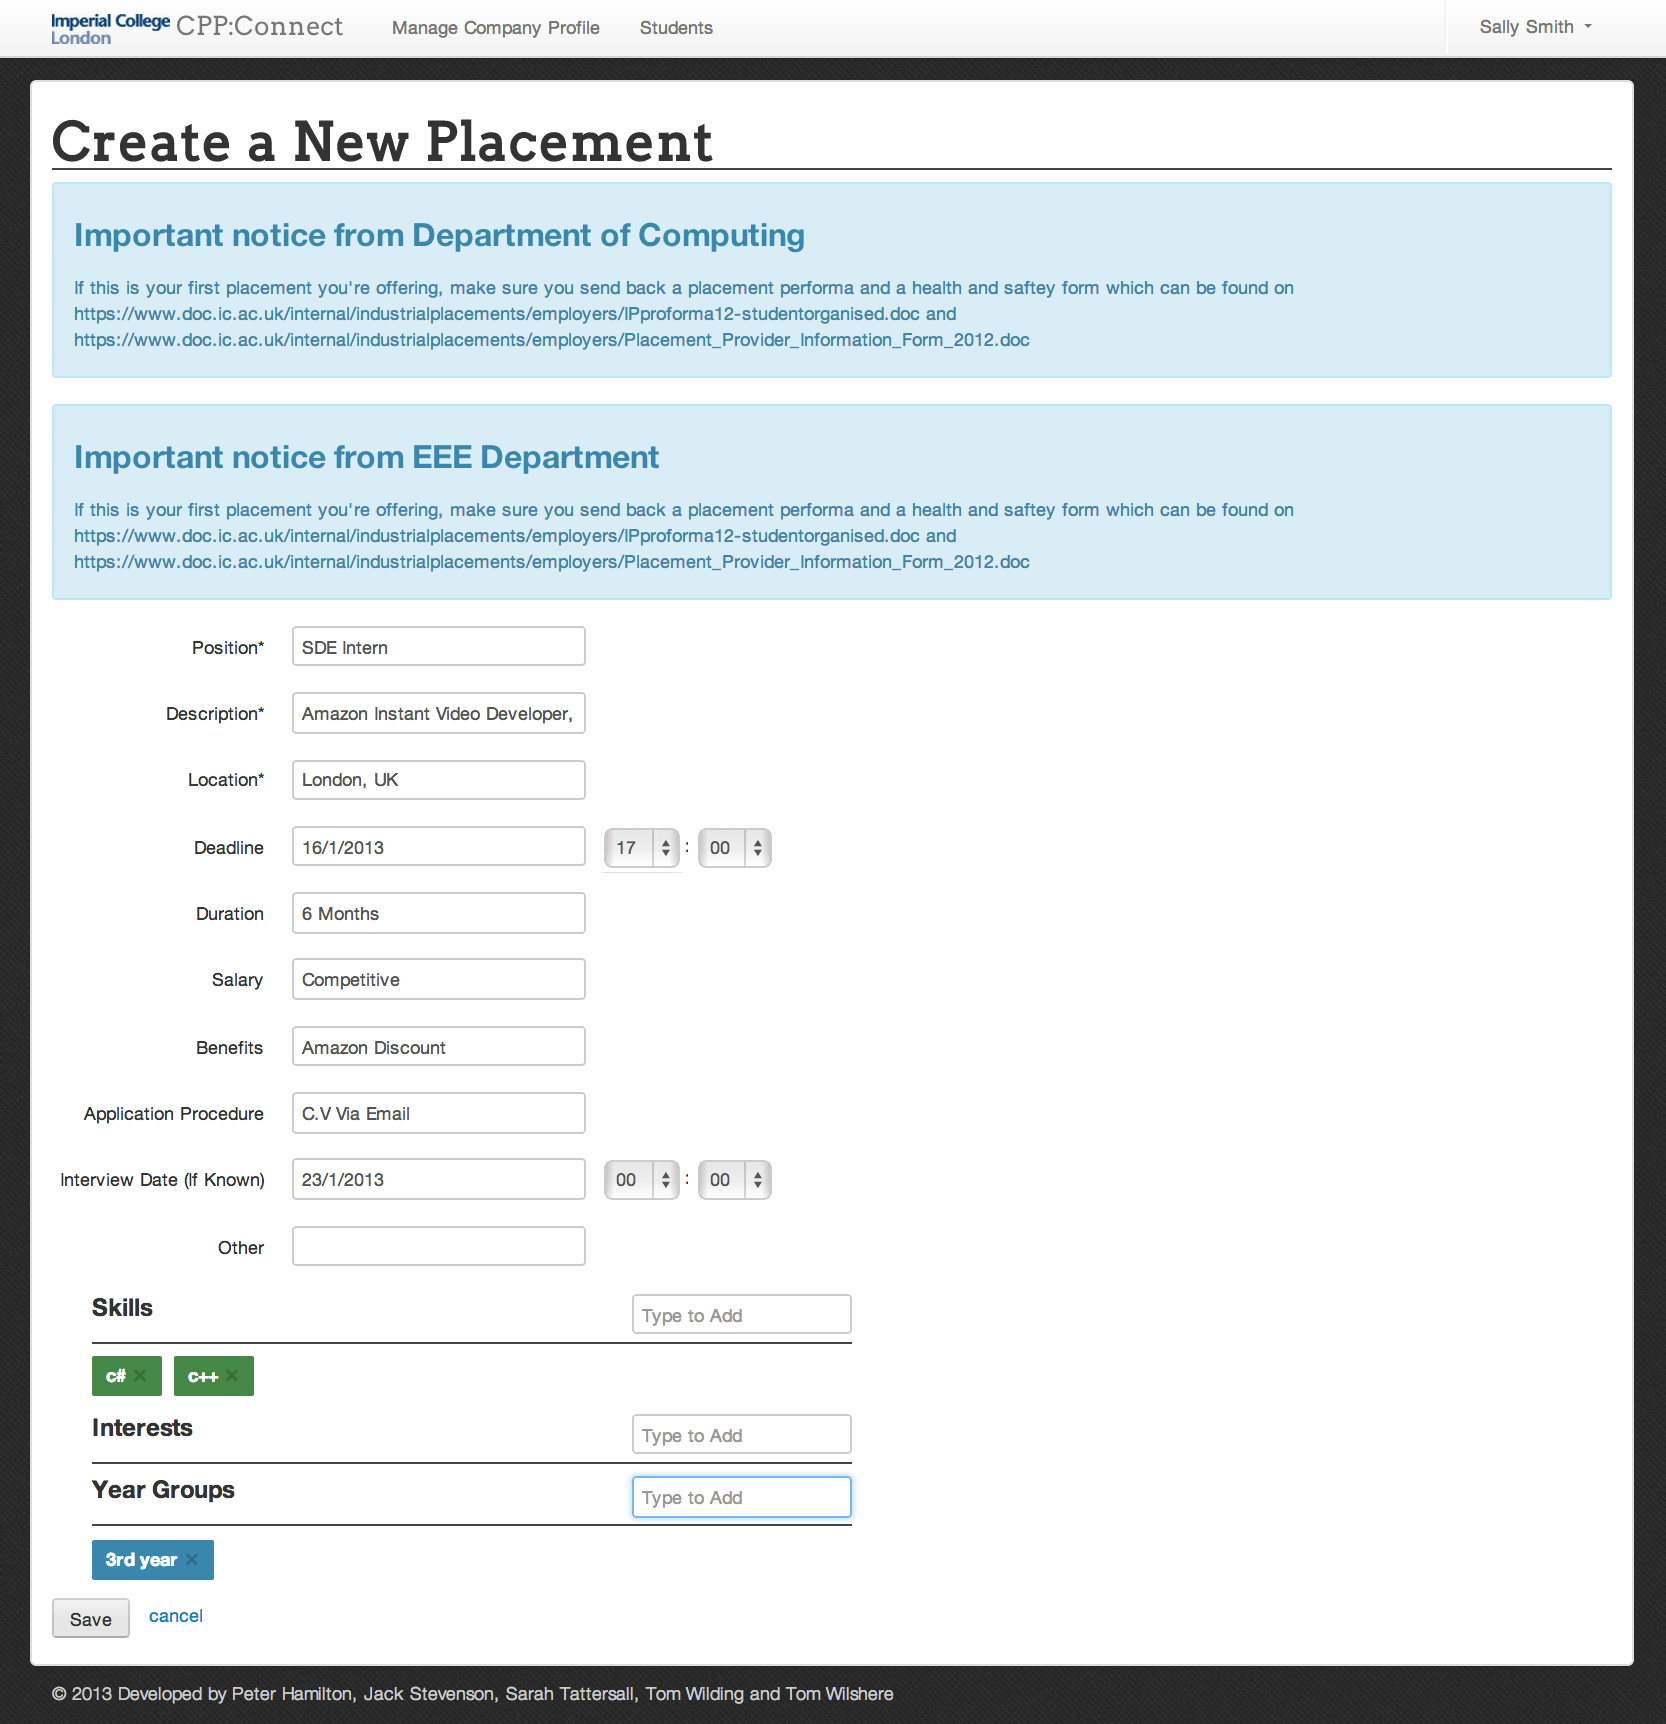
\includegraphics[scale=0.5]{images/user_experiences/company/new_placement}
    \caption{Creating a company placement}
    \end{figure}

    Similarly she can do the exact same thing with events.

    If Sally later decides to look at an event that Amazon is already advertising, she has the option to email the students with some useful information, like how to get to Amazon from the tube station.
    This email will only be sent to recipients that are actually attending the event and must receive approval by a department administrator before it is actually sent.

    \begin{figure}[H]\centering
    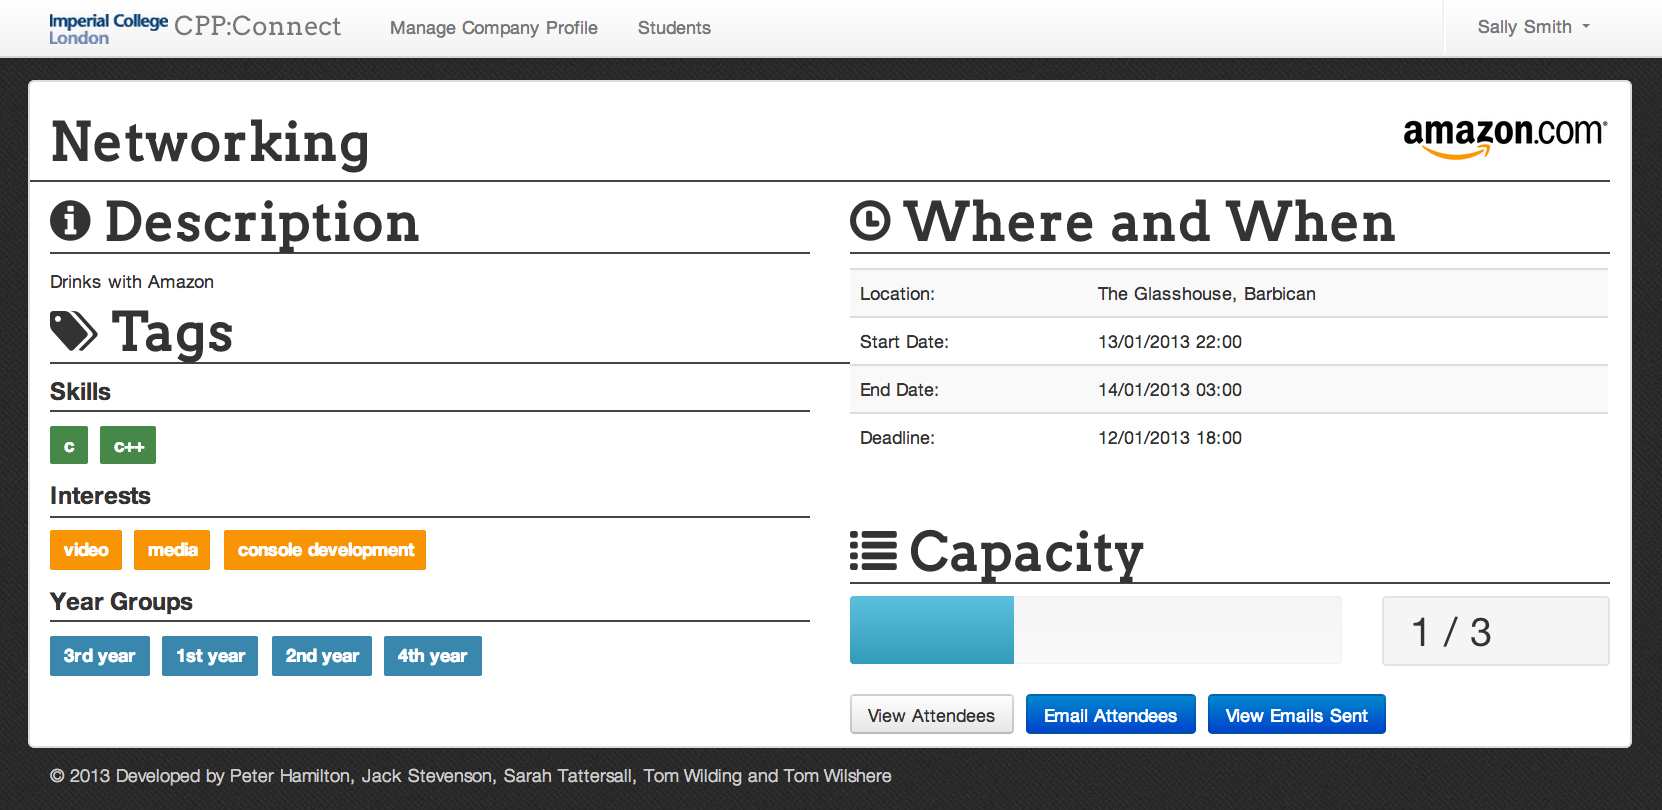
\includegraphics[scale=0.5]{images/user_experiences/company/networking_event}
    \caption{Companies can view and contact students attending events}
    \end{figure}

    There is also a `view attending students' button so that Sally can view who is planning to attend. We feel this feature might be more relevant after an event so that if a particular student stood out to her she can look them up online.

  \paragraph{Students:}
    After creating placements and events Sally decides she wants to browse all students to find exceptional candidates she can contact herself. She clicks on students on the navigation bar and is greeted by a list of students. Note that any students who have decided to blacklist Amazon will never appear in this list, nor will deactivated students.
    Since she knows Amazon will be recruiting for C++ developers, she specifically types C++ into the skills filter
    and browses the updated list of students.

    \begin{figure}[H]\centering
    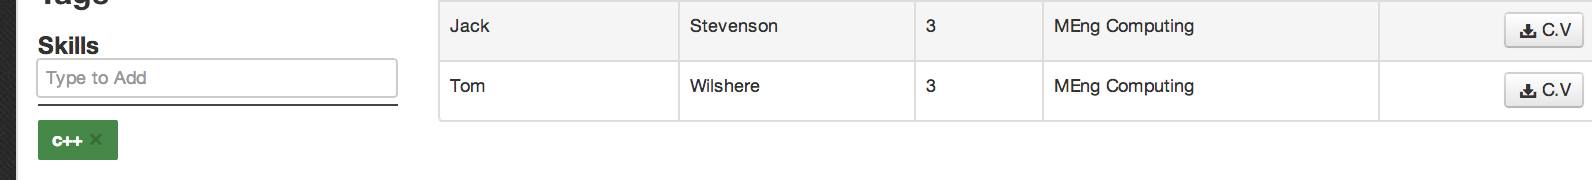
\includegraphics[scale=0.5]{images/user_experiences/company/c++_student_search}
    \caption{Company search of students with C++ skill}
    \end{figure}

    She can then browse their profile `cards', which are a reduced version of the student view, lacking the events and placement sections since they are not relevant to companies. Since Jack has listed C++ as a skill his profile appears on the list.

    \begin{figure}[H]\centering
    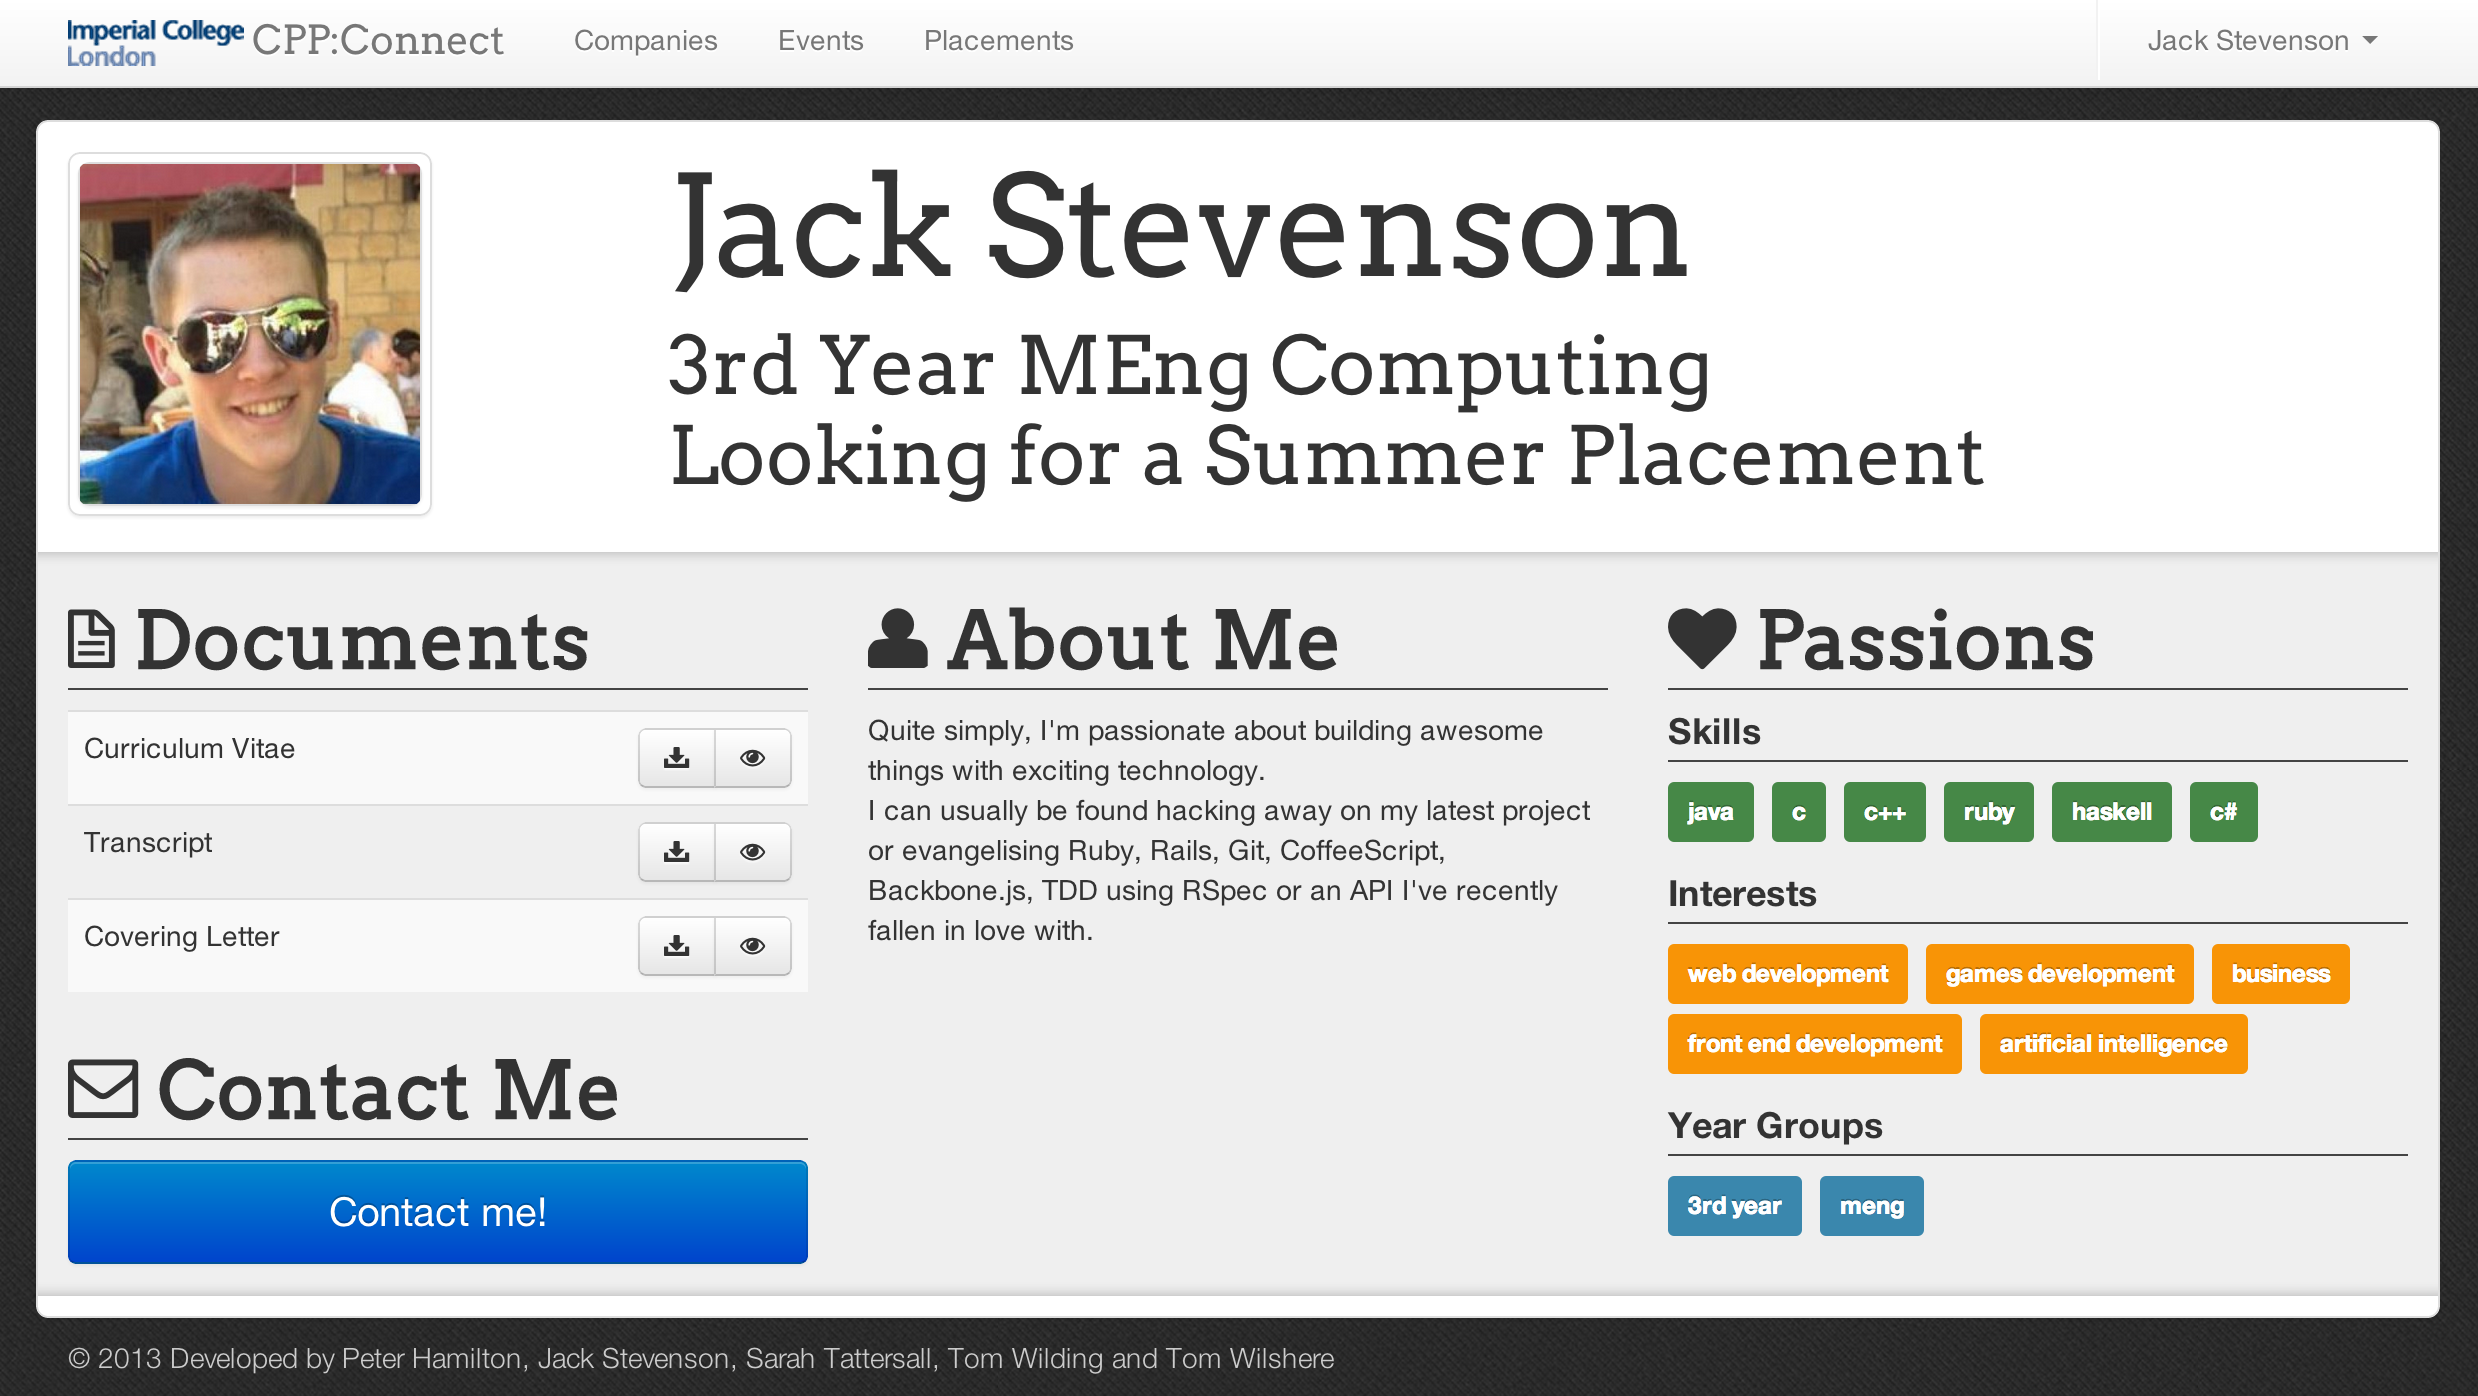
\includegraphics[scale=0.3]{images/user_experiences/company/jack_profile}
    \caption{Company view of student profile}
    \end{figure}

    Liking what she sees, Sally can then choose to download Jack's CV to her computer or view it online with the preview icon button. After reading Jack's CV Sally then chooses to invite Jack to interview by clicking on the `contact me' button which we have made large to make it clear to companies we would like them to contact students. She then sends an email from her account to his address which he can reply to if he wants.


    \begin{figure}[H]\centering
    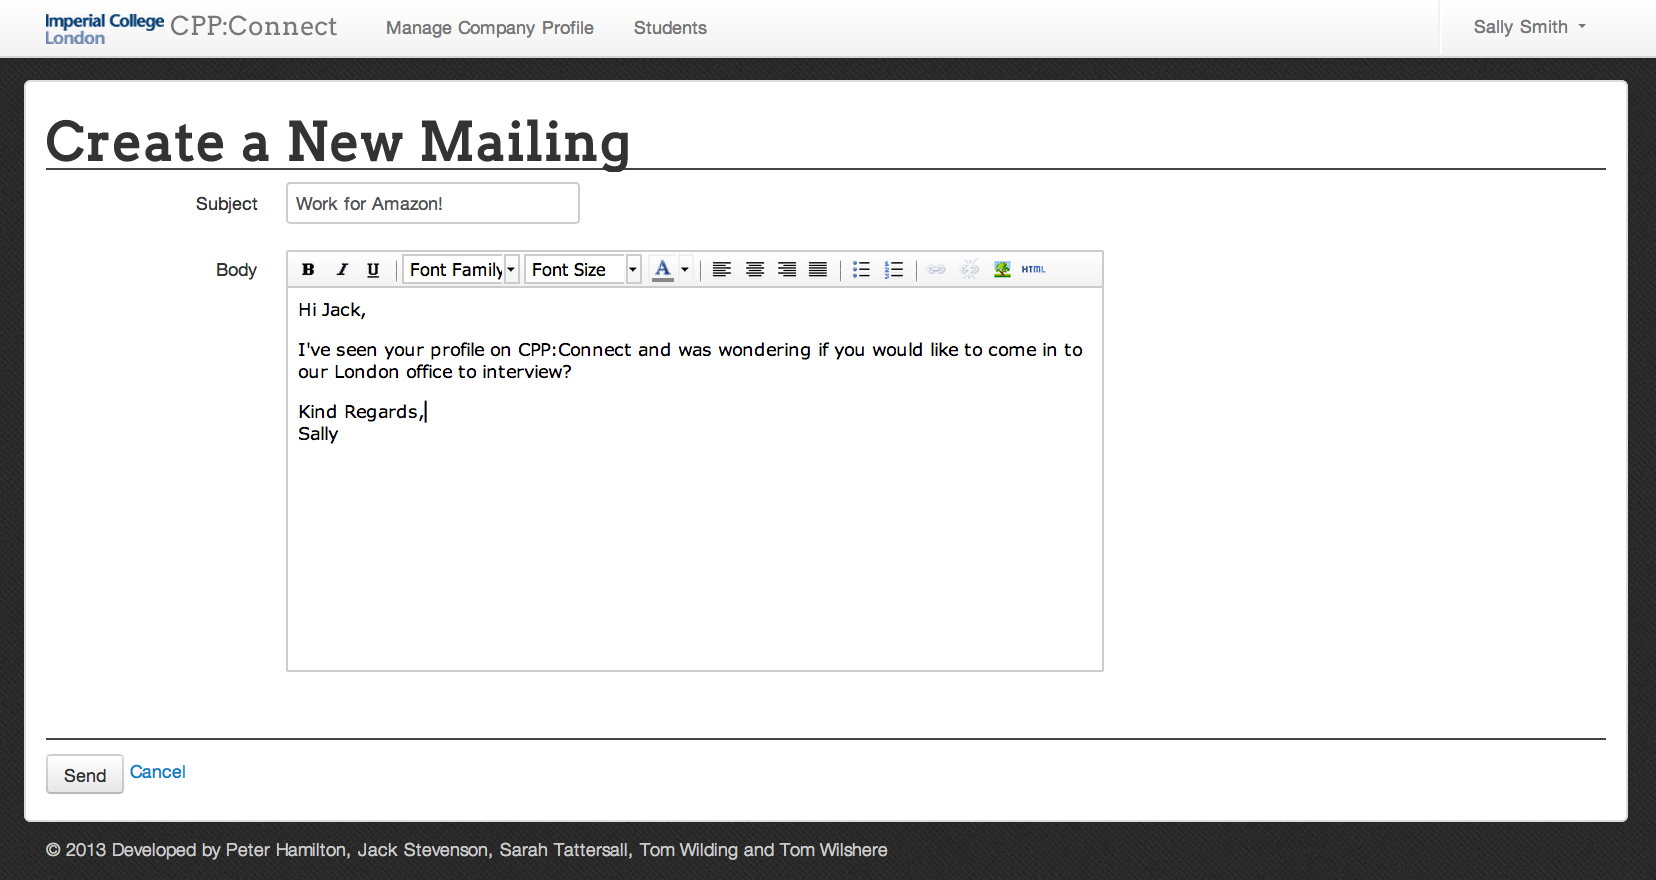
\includegraphics[scale=0.3]{images/user_experiences/company/jack_offer_email}
    \caption{Company can send students personal emails}
    \end{figure}

    If a student gets fed up with receiving personal emails from any company, their blocking feature easily ensures that they can never contact them again.

  \paragraph{Emails:}
    Being a member of the Corporate Partnership Programme entitles Amazon to be able to contact a departments' students via email. Sally can create emails to inform students of exciting scholarships and other opportunities Amazon are offering. The great thing about our email client is that it supports HTML, so company styles can be used when sending emails through our system. Many companies use HTML emails with rich content when emailing students at the moment so this will allow that practice to continue, and indeed encourages companies to spend more time making their emails look enticing.

    We have chosen for emails to be approved by an administrator to avoid companies being able to spam students and we hope that the need for administrator approval encourages them to write detailed informative emails that are of an appropriate content for students. If it is not deemed applicable enough the administrator can send the email back to the company for modification specifying a reason, or reject it outright.
    We do not at current require approval for direct (personal) emails to students as this is deemed too much work for a CPP administrator.


    %%%%%%%%%%%%%%%%%%%%%%%%%%%% TODO %%%%%%%%%%%%%%%%%%%%%%%%%%%%%
    % * Companies requesting permissions for students, perhaps Sally wants Maths students?
    % * Print screens
    % * Describe a little more about the emails
    %%%%%%%%%%%%%%%%%%%%%%%%%%%%%%%%%%%%%%%%%%%%%%%%%%%%%%%%%%%%%%%
